\documentclass[a4paper,UTF8]{article}
\usepackage{ctex}
\usepackage[margin=1.25in]{geometry}
\usepackage{color}
\usepackage{graphicx}
\usepackage{amssymb}
\usepackage{amsmath}
\usepackage{amsthm}
\usepackage{listings}
\usepackage{subfigure}
%\usepackage[thmmarks, amsmath, thref]{ntheorem}
\theoremstyle{definition}
\newtheorem*{solution}{Solution}
\newtheorem*{prove}{Proof}
\usepackage{multirow}
\usepackage{url}
\usepackage[colorlinks,urlcolor=blue]{hyperref}
\usepackage{enumerate}
\usepackage{xcolor}
\lstset{
    %backgroundcolor=\color{red!50!green!50!blue!50},%代码块背景色为浅灰色
    rulesepcolor= \color{gray}, %代码块边框颜色
    breaklines=true,  %代码过长则换行
    numbers=left, %行号在左侧显示
    numberstyle= \small,%行号字体
    %keywordstyle= \color{red},%关键字颜色
    commentstyle=\color{gray}, %注释颜色
    frame=shadowbox%用方框框住代码块
    }
\renewcommand\refname{参考文献}


%--

%--
\begin{document}
\title{\textbf{《计算机图形学》10月报告}}
\author{171850505,宋昱豪,\href{mailto:yhsong.nju@gmail.com}{yhsong.nju@gmail.com}}
\maketitle

\section{综述}
基于计算机图形学设计了一套画图系统。完成了画图软件。主要实现了基于各种算法的图元生成,图元编辑,文件的保存打开,基于文档文件的指令序列读取完成画图任务,基于鼠标交互的图元绘制。并在此基础上对于软件界面进行了美化,具有一定可用性。\\
\\ \textbf{关键词:} openGL \qquad  Qt gui设计 \qquad 计算机图形学
\section{算法介绍}
\subsection{直线绘制算法}
\subsubsection{DDA算法}
数字差分分析法(Digital Differential Analyzer, DDA)是利用计算两个坐标方向的差分来确定线段显示的屏幕像素位置的线段扫描转换算法。DDA算法的核心是增量式的思想。即利用光栅的特性消除了直线方程中的乘法,在x和y方向使用合适的增量来逐步沿直线的路径推导出各像素的位置。
\par 现假设直线的方程为
\begin{equation}
y=m\times x +b
\end{equation}
\par 假设斜率$m \leq 1$,在x的维度上单位间隔采样并求每个采样点对应的y值,可以发现在对于$x_{k+1}=x_{k}+1$的x采样时,$y_{k+1}=y_{k}+m$。因此在屏幕光栅的特点下,我们采用增量式的方法计算出直线路径上各像素点的位置。而当斜率$m \textgreater 1$时,我们在y的维度上进行采样,对于$y_{k+1}=y_{k}+1$时,$x_{k+1}=x_{k}+\frac {1}{m}$。在起始点和终点位置不同时增量的符号可能会改变。
\subsubsection{Bresenham算法}
在DDA算法中,由于斜率为浮点数,而浮点增量的连续迭加中取整误差的积累会使得计算得到的像素位置与实际上的像素位置偏离。同时浮点计算也十分耗时。而Bresenham算法通过引入整形参量定义来衡量两候选像素与直线路径上实际点在方向上的偏移。并通过对该参量的符号判定来决定像素点的选择。
\begin{figure}[ht]
\centering
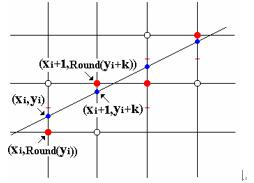
\includegraphics[width=13cm]{x1.jpg}
\caption{Brensenham 示意图}
\label{x1}
\end{figure}
\par 假设依然以x的维度为基础,设目前已经绘制到第k步在点($x_{k}$,$y_{k}$),下一个点的位置在($x_{k+1}$,$y_{k}$)或者($x_{k+1}$,$y_{k+1}$)。由于点$x_{k+1}$处y的值可以表示为

\begin{equation}
y = m \times x_{k+1} + b =m \times (x_{k}+1)+b
\end{equation}

\par 此时两个候选的像素和线段的数学路径的垂直偏移为

\begin{equation}
\left\{
\begin{aligned}
d_{1}=y-y_{k}=m \times (x_{k}+1)+b-y_{k}\\
d_{2}=y_{k+1}-y=y_{k}+1-m \times (x_{k}+1)+b\\
\end{aligned}
\right.
\end{equation}
\par 这两个点距离理想点的距离的差分为

\begin{equation}
d_{1}-d_{2}=2 \times (x_{k}+1)-2 \times y_{k}+2 \times b -1
\end{equation}

\par 为了达到消除浮点数运算的目的,令$m=frac{\Delta y}{\Delta x}$,设变量
\begin{equation}
p_{k}=\Delta x (d_{1}-d_{2})=2\Delta y x_{k}-2\Delta x y_{k}+c
\end{equation}
\par 同时由于c为常数,所以在循环计算中被消除,因为$\Delta x=1 \textgreater 0$,所以$p_{k}$的符号与$d_{1}-d_{2}$的符号相同。当$y_{k}$处的像素点比$y_{k+1}$处的像素点更加接近理想线段时,$p_{k}<0$,反之则大于零。所以我们可以根据$p_{k}$的符号来决定k+1步走到的位置。
\par 

\subsection{圆形绘制算法}
采用中点圆生成算法,为了简化运算,只计算出八分之一的圆上的点,其他的点由计算单得到的八分之一圆旋转对称得到。
\begin{figure}[ht]
\centering
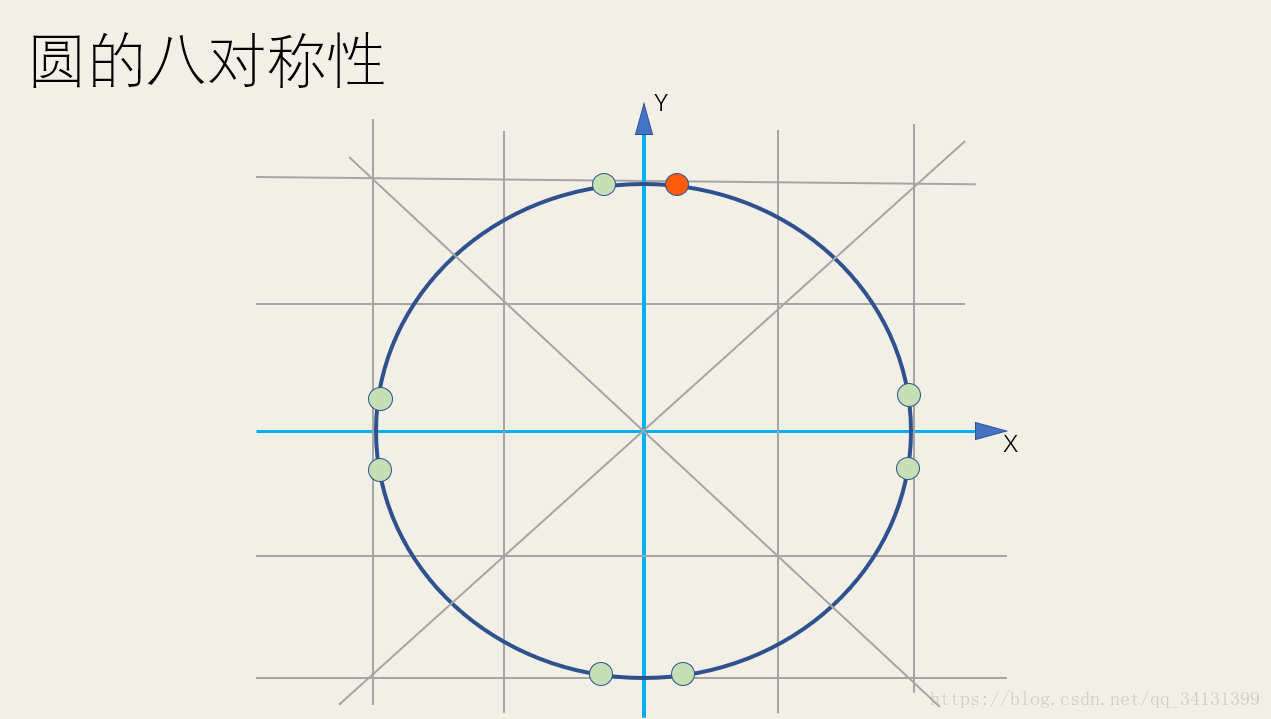
\includegraphics[width=12cm]{x2.png}
\caption{圆的对称性 示意图}
\label{x2}
\end{figure}
\par 在中点圆算法中,和画直线的Bresenham算法类似,判断的参数是由点到中心的距离计算得到的。计算的是两个候选点的中点到圆心的距离。
\begin{equation}
\left\{
\begin{aligned}
p_{k+1}=f_{circle}(x_{k+2},y_{k}-frac{1}{2}) \qquad p_{k}<0\\
p_{k+1}=f_{circle}(x_{k+2},y_{k}-frac{3}{2}) \qquad p_{k}\geq 0
\end{aligned}
\right.
\end{equation}
\par 计算推导可得
\begin{equation}
\left\{
\begin{aligned}
p_{k+1}=p_{k}+2x_{k}+3 \qquad p_{k}<0\\
p_{k+1}=p_{k}+2x_{k+1}-2y_{k}+5 \qquad p_{k}\geq 0
\end{aligned}
\right.
\end{equation}
\par 在计算中设置$p_{0}$为$5-4\times r$ 初始化第一个点为(0,r)开始计算

\begin{figure}[ht]
\centering
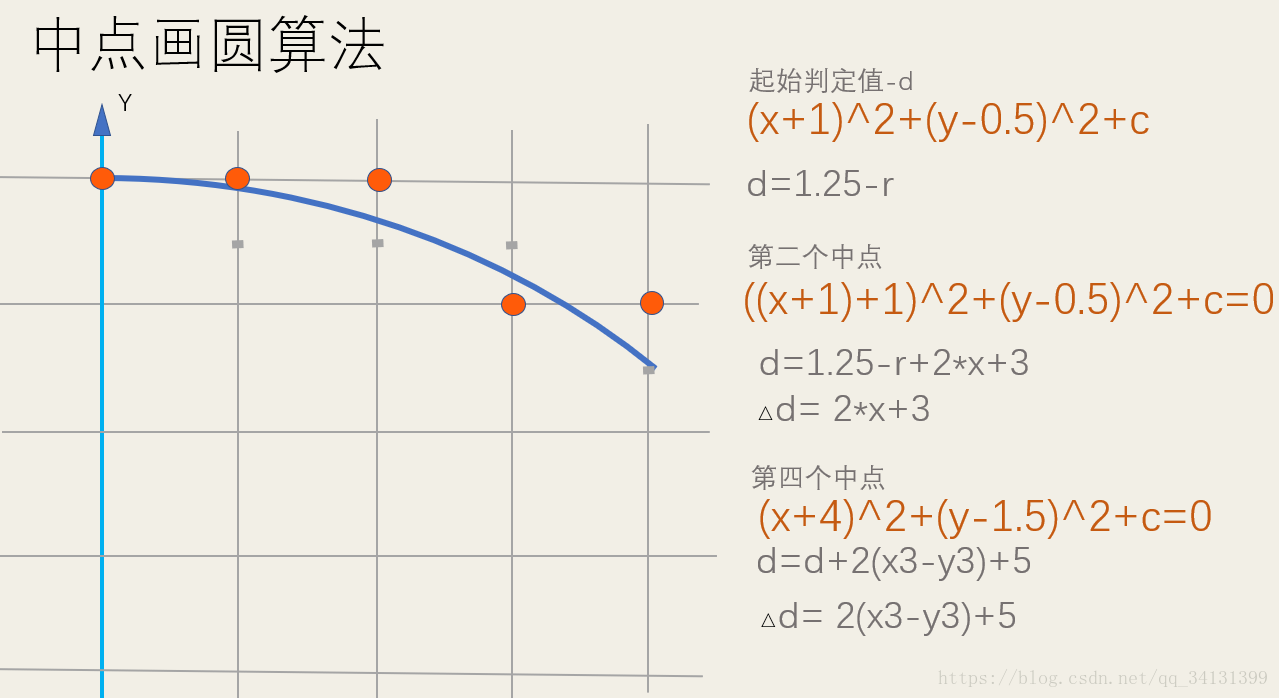
\includegraphics[width=13cm]{x3.png}
\caption{中点圆画法 示意图}
\label{x3}
\end{figure}
\subsection{中点椭圆绘制算法}
椭圆绘制算法类似于中点圆生成算法,但是中点椭圆绘制算法中只能计算出四分之一的图形,剩下的用对称可以得到。在这四分之一图形中我们又要分成两个部分来计算点的位置。我们以一个以原点为中心的椭圆为例,我们只需要计算其第一象限内的点的位置。
\begin{figure}[ht]
\centering
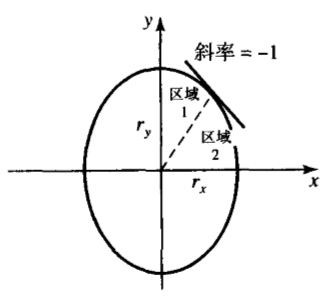
\includegraphics[width=7cm]{x4.png}
\caption{椭圆对称性 示意图}
\label{x4}
\end{figure}
区域一即为其切线斜率小于1的部分,区域二为大于1的部分。
在区域一中,我们有参数
\begin{equation}
\left\{
\begin{aligned}
p_{k+1}=p_{k}+2r_{y}^2 x_{k}+3 r_{y}^2 \qquad p_{k}<0\\
p_{k+1}=p_{k}+2r_{y}^2x_{k+1}-2r_{x}^2 y_{k}+3 r_{y}^2 \qquad p_{k}\geq 0
\end{aligned}
\right.
\end{equation}
\par 在区域二中参数变化为
\begin{equation}
\left\{
\begin{aligned}
p_{k+1}=p_{k}-2r_{x}^2 y_{k}+3 r_{x}^2 \qquad p_{k}<0\\
p_{k+1}=p_{k}+2r_{y}^2x_{k+1}-2r_{x}^2 y_{k}+3 r_{x}^2 \qquad p_{k}\geq 0
\end{aligned}
\right.
\end{equation}
\begin{figure}[ht]
\centering
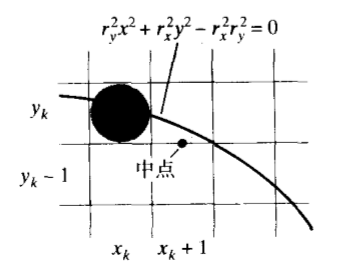
\includegraphics[width=7cm]{x5.png}
\caption{中点椭圆画法 示意图}
\label{x5}
\end{figure}
\subsection{矩形绘制算法}
矩形绘制算法即根据获得到的两个点的坐标,分别作为矩形对角线的两个端点,生成其他端点并调用画线算法即可完成。
\begin{figure}[ht]
\centering
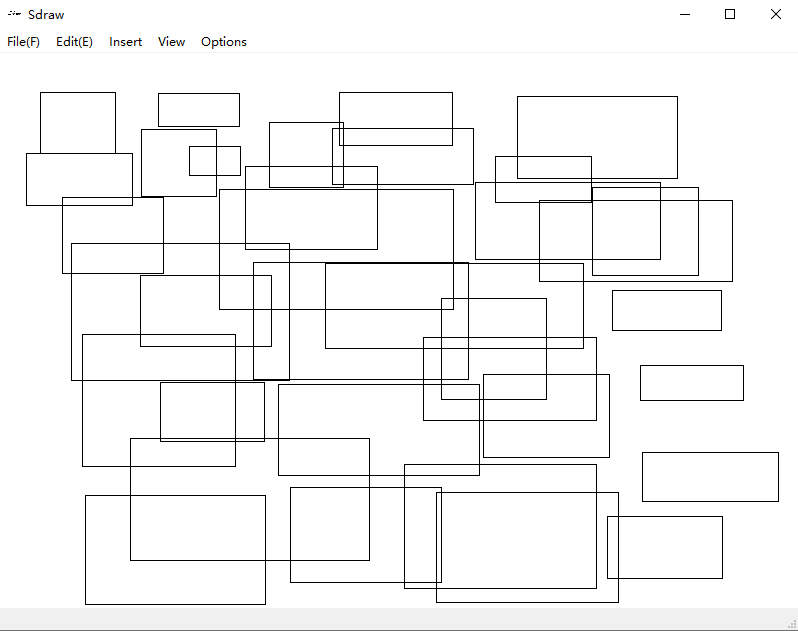
\includegraphics[width=7cm]{x6.png}
\caption{矩阵 示意图}
\label{x6}
\end{figure}
\subsection{曲线算法}
此软件中实现了两种曲线绘制算法,即贝塞尔曲线和B样条曲线
\subsubsection{贝塞尔曲线}
\begin{figure}[ht]
\centering
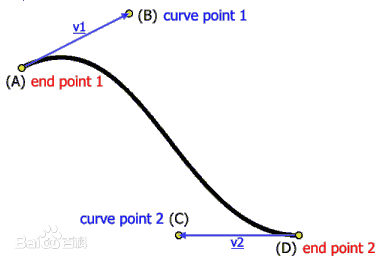
\includegraphics[width=6cm]{x15.jpg}
\caption{贝塞尔曲线画法 示意图}
\label{x5}
\end{figure}
\par
Bézier curve(贝塞尔曲线)是应用于二维图形应用程序的数学曲线。 曲线定义:起始点、终止点(也称锚点)、控制点。通过调整控制点,贝塞尔曲线的形状会发生变化。 1962年,法国数学家Pierre Bézier第一个研究了这种矢量绘制曲线的方法,并给出了详细的计算公式,因此按照这样的公式绘制出来的曲线就用他的姓氏来命名,称为贝塞尔曲线。
\par Bezier曲线是参数多项式曲线,它由一组控制多边形折线(控制多边形)的顶点唯一定义,在控制多边形的各顶点中,只有第一个和最后一个顶点在曲线上,其他的顶点则用以定义曲线的导数,阶次和形状。Bezier曲线的数学基础是能够在第一个和最后一个顶点之间进行插值的一个多项式混合函数,对于有n+1个控制点的Bezier曲线段用参数方程表示如下:
\begin{equation}
P(t)=\sum_{k=0}^n P_{k} BEN{k,n}(t)\qquad t\in [0,1]
\end{equation}
式中$P_{k}(x_{k},y_{k},z_{k})$,k=0,1,2…..n是控制多边形的n+1个顶点,$BEN_{k,n}$(t)是Bernstein基函数。
\begin{equation}
 BEN{k,n}(t)=\frac{n!}{k!*(n-k)!} *t^k*(1-t)^{n-k}
\end{equation}
\subsubsection{B样条曲线}
B-样条是贝塞尔曲线的一种一般化,B样条不能表示一些基本的曲线,比如圆,所以引入了NURBS,可以进一步推广为非均匀有理B-样条(NURBS)。三者关系可以表示为:
\begin{figure}[ht]
\centering
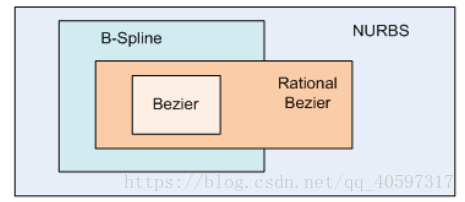
\includegraphics[width=6cm]{x16.png}
\caption{曲线包含关系 示意图}
\label{x16}
\end{figure}
\par 给定n+1个控制点,$P_{0},P_{1}, ..., P_{n}以及一个节点向量U={u_{0},u_{1}, ..., u_{m}}$, p次B样条曲线由这些控制点和节点向量U 定义,其公式为:
\begin{equation}
C(u) = \sum_{i=0}^n N_{i,p}(u)P_{i}
\end{equation}
\par 上式中,$N_{i,p}(u)$为B样条基函数
\par 设U 是m+1个非递减数的集合,$u_{0}<=u_{1}<=u_{2}<= ... <= u_{m}。u_{i}$称为节点(knots), 集合U 称为节点向量(knot vector), 半开区间$[u_{i}, u_{i+1})$ 是第i个节点区间(knot span)。注意某些$u_{i}$可能相等,某些节点区间会不存在。如果一个节点$u_{i}$出现 k 次 (即,$u_{i} = u_{i+1} = ... = u_{i+k-1}$), 其中 k > 1, ui 是一个重复度(multiplicity)为k 的多重节点,写为 $u_{i}(k)$。 否则,如果$u_{i}$只出现一次,它是一个简单节点。如果节点等间距(即,$ u_{i+1} - u_{i} $是一个常数,对 0 <= i <= m - 1),节点向量或节点序列称为均匀的;否则它是非均匀的。一般情况下,我们经常使用 $u_{0} = 0和 u_{m} = 1$,所以定义域是闭区间[0,1]。
\par 为了定义B-样条基函数,我们还需要一个参数,基函数的次数(degree)p,第i个p次B-样条基函数,写为$N_{i,p}(u)$,递归定义如下:
\begin{equation}
N_{i,0}(u)=
\left\{
\begin{aligned}
1 \qquad if u_{i} \leq u \leq u_{i+1} \\
0 \qquad otherwise
\end{aligned}
\right.
\end{equation}

\begin{equation}
N_{i,p}(u)= \frac{u-u_{i}}{u_{i+p}-u_{i}}N_{i,p-1}(u)+\frac{u_{i+p+1}-u}{u_{i+p+1}-u_{i+1}}N_{i+1,p-1}(u)
\end{equation}
\subsection{选中算法}
选中即为,当用户鼠标点击的坐标所对应的像素点时,如果该像素点对应于画布上的图元,则选中该图元。选中算法为了用户操作的鲁棒性,当用户点击的坐标附近一定参数范围内存在相应的图元时,则选中该图元。程序中搜索相应图元位置则是在画图的画板中遍历搜索,当搜索到第一个距离点击点在操作范围内的图元时,则将标志变量choosenid标志为该图元的图元编号,同时将ischoose flag设置为true,表示成功选中了图元,在paintGL中,每次刷新画图时,如果发现当前遍历到的图元被选中的话,则将该图元颜色变化为灰色。
\begin{figure}[htbp]
\centering    %居中
 
\subfigure[原图] %第一张子图
{
	\begin{minipage}[t]{0.35\linewidth}
	\centering          %子图居中
	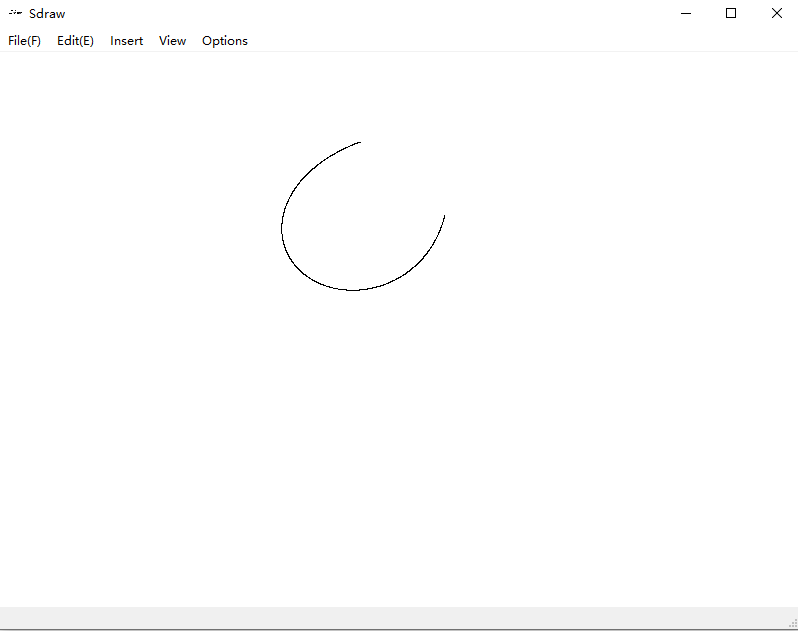
\includegraphics[width=6cm]{x11.png}   %以pic.jpg的0.5倍大小输出
	\end{minipage}
}
\subfigure[选中后] %第二张子图
{
	\begin{minipage}[t]{0.35\linewidth}
	\centering      %子图居中
	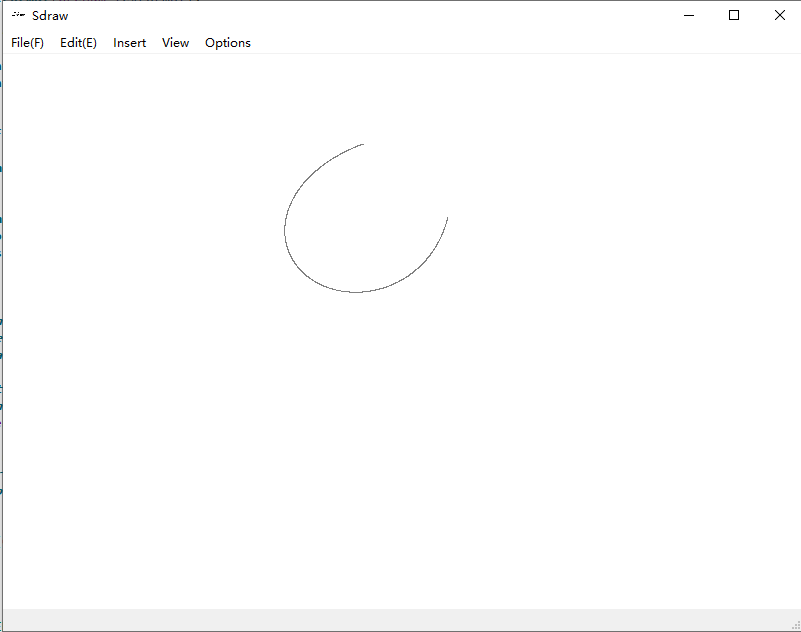
\includegraphics[width=6cm]{x12.png}   %以pic.jpg的0.5倍大小输出
	\end{minipage}
}
 
\caption{选中算法 示意图} %  %大图名称
\label{x1112}  %图片引用标记
\end{figure}
\subsection{删除算法}
删除算法是在图形化界面中的服务的功能。在图形界面中必须基于选中算法来完成,该算法即遍历画布中所有的像素点,如果像素点的状态为选中,则从画布集合中删除该点。
\subsection{移动算法}
移动算法的完成较为简单,在图形界面中是依赖于选中算法来完成的,首先遍历画布集合中所有的点,如果发现有像素点的状态为选中,则将其位置加上参数需要的偏移量。在读文件操作中偏移量是已经给出的。但是在图形化界面中,偏移量是由用户操作完成的,所以我们设定用户一次点击释放鼠标左键为一次移动完成,开始点即为用户press左键所在的位置,结束的位置即为用户release鼠标左键所在的位置。用开始结束的位置信息来计算移动向量。传给移动函数,完成移动函数。
\begin{figure}[htbp]
\centering    %居中
 
\subfigure[原图] %第一张子图
{
	\begin{minipage}[t]{0.35\linewidth}
	\centering          %子图居中
	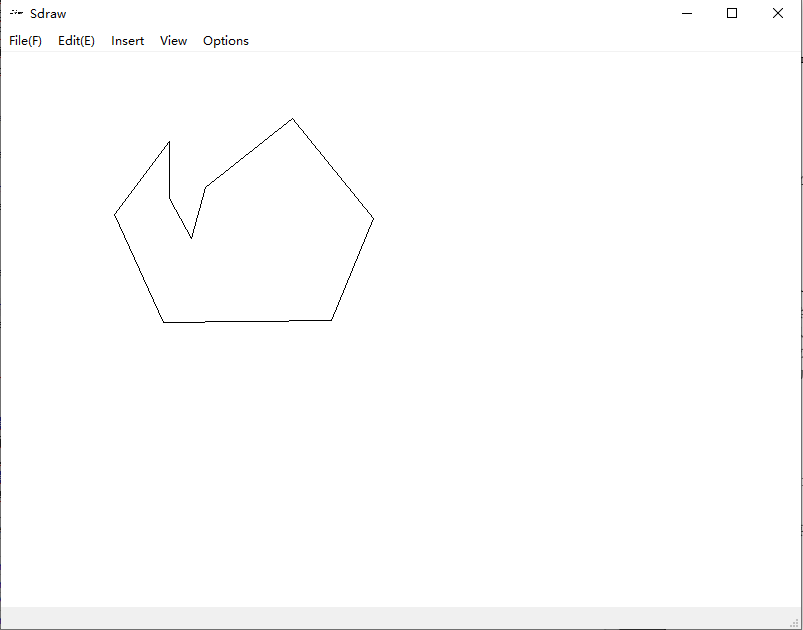
\includegraphics[width=6cm]{x13.png}   %以pic.jpg的0.5倍大小输出
	\end{minipage}
}
\subfigure[移动后] %第二张子图
{
	\begin{minipage}[t]{0.35\linewidth}
	\centering      %子图居中
	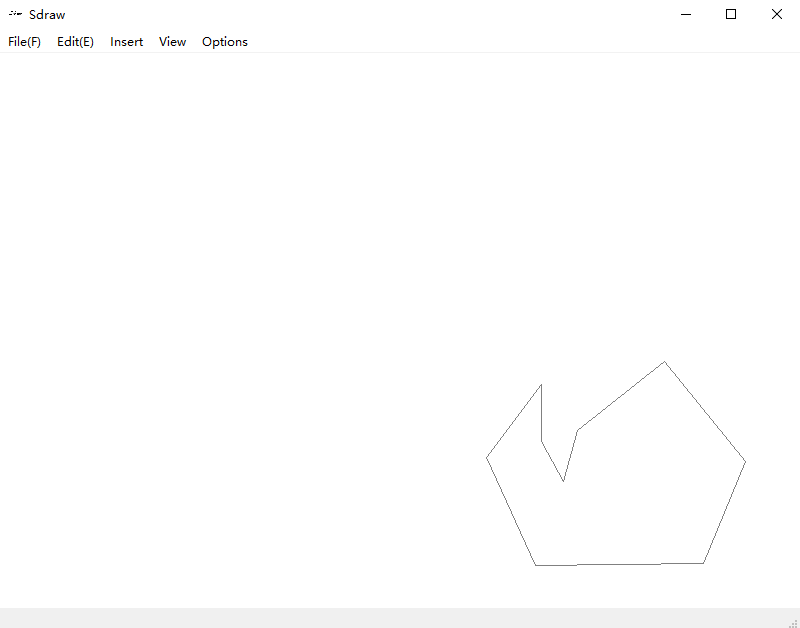
\includegraphics[width=6cm]{x14.png}   %以pic.jpg的0.5倍大小输出
	\end{minipage}
}
 
\caption{移动算法 示意图} %  %大图名称
\label{x1314}  %图片引用标记
\end{figure}
\subsection{裁剪算法}
\par 裁剪算法由两种算法完成:
\subsubsection{CohenSutherland}
\par Cohen-Sutherland 算法是最早、最流行的线段裁剪算法,核心思想是通过编码测试来减少要计算交点的次数。线段端点按区域赋以四位二进制码(区域码)。
\par 区域码各位从右到左编号:
\par 位1:上边界。
\par 位2:下边界。
\par 位3:右边界。
\par 位4:左边界。
\par 区域码位=1:端点落在相应位置上,区域码位=0:端点不在相应位置上。
\par
\begin{figure}[ht]
\centering
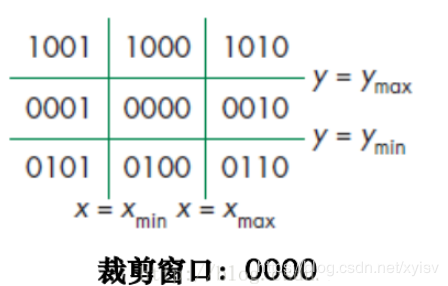
\includegraphics[width=10cm]{s1.png}
\caption{编码}
\label{s1}
\end{figure}
\par
\par 区域码位值通过将端点坐标值(x,y)与裁剪窗口边界坐标比较来确定。根据线段端点的区域码快速判断:1. 完全在窗口边界内的线段:两端点区域码均为0000;2.完全在裁剪矩形外的线段:两端点区域码同样位置都为1;对两个端点区域码进行逻辑与操作,结果不为0000。不能确定完全在窗口内外的线段,进行求交运算:按“左-右-上-下”顺序用裁剪边界检查线段端点:将线段的外端点与裁剪边界进行比较和求交,确定应裁剪掉的线段部分;反复对线段的剩下部分与其它裁剪边界进行比较和求交,直到该线段完全被舍弃或找到位于窗口内的一段线段为止。
\par 在程序的代码实现上,发现问题是在求交操作上,由于像素点在屏幕上的离散分布,所以程序求得的交点很可能不在原本的直线上,而且即使在原本的直线上,裁剪重新得到的直线与原本直线也可能不重合,所以在程序中需要使用删除原本的图元再重新画的操作。在计算交点逐步裁剪的过程中使用一个while循环,每次裁剪一段,直到直线的两端都在区域0000时结束。
\par 

\subsubsection{Liang-barsky}
\par 设要裁剪的直线段为$P_{0}$ $P_{1}$, $P_{i}$的坐标为$(x_{i},y_{i})$,i=0, 1。 $P_{0} P_{1}$和窗口边界交于A、B、C和D四个点。我们知道,一条两端点为$P_{1}(x_{1},y_{1})、P_{2}(x_{2},y_{2})$的线段可以用参数方程形式表示: 
\begin{equation}
\left\{
\begin{aligned}
x=x_{1}+u(x_{2}-x_{1})=x_{1}+u\delta x\\
y=y_{1}+u(y_{2}-y_{1})=y_{1}+u\delta y
\end{aligned}
\right.
\end{equation}


\begin{figure}[ht]
\centering
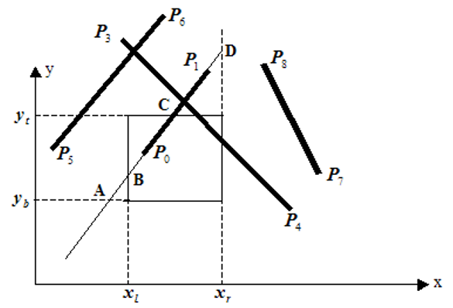
\includegraphics[width=10cm]{s2.png}
\caption{交点}
\end{figure}

\label{s2}
\par 式中,$\delta x=x_{2}-x_{1}$,$\delta y=y_{2}-y_{1}$,参数u在0~1之间取值,P(x,y)代表了该线段上的一个点,其值由参数u确定,由公式可知,当u=0时,该点为$P_{1}(x_{1},y_{1})$,当u=1时,该点为$P_{2}(x_{2},y_{2})$。如果点P(x,y)位于由坐标$(x_{min},y_{min})和(x_{max},y_{max})$所确定的窗口内,那么下式成立:
\begin{equation}
\left\{
\begin{aligned}
x_{min}\leq x_{1}+u\delta x\leq x_{max}\\
y_{min}\leq y_{1}+u\delta y\leq y_{max}
\end{aligned}
\right.
\end{equation}
\par 这四个不等式可以表示为:
\begin{equation}
u*p_{k}\leq q_{k}\qquad k=1,2,3,4
\end{equation}
\par 任何平行于窗口某边界的直线,其pk=0,k值对应于相应的边界(k=1,2,3,4对应于左、右、下、上边界)。
\par 如果$q_{k}<0$,则线段完全在边界外,应舍弃该线段。
\par 如果$q_{k}\geq 0$,则线段平行于窗口某边界并在窗口内。
\par 所以,当pk<0时,线段从裁剪边界延长线的外部延伸到内部;当pk>0时,线段从裁剪边界延长线的内部延伸到外部。
\par 对于每条直线,可以计算出参数u1和u2,该值定义了位于窗口内的线段部分:\\
1.u1的值由线段从外到内遇到的矩形边界所决定(pk<0),对这些边界计算rk=qk/pk,u1取0和各个r值之中的最大值。
2.u2的值由线段从内到外遇到的矩形边界所决定(pk>0),对这些边界计算rk=qk/pk,u2取1和各个r值之中的最小值。
3.如果u1>u2,则线段完全落在裁剪窗口之外,应当被舍弃;否则,被裁剪线段的端点可以由u1和u2计算出来。
\par 

\subsection{旋转算法}
旋转算法实现的是刚性旋转,所以我们只需要旋转改变图元的构造点,即对构造点进行操作。所以我们需要改变之前存储图元的方式,为了方便接下来此类操作,我们创造了一个图元字典,存储了图元的构造点数据,图元编号,图元所属模式等等属性。所以当需要对图元进行构造上的操作改变时,只需要从字典中检索即可。旋转算法只需要将原本的坐标乘一个矩阵,便可以得到所需要的新的点的位置。
\begin{equation}
\left\{
\begin{aligned}
x=x_{r}+(x-x_{r})cos(\theta)-(y-y_{r})sin(\theta)\\
y=y_{r}+(x-x_{r})sin(\theta)+(y-y_{r})cos(\theta)
\end{aligned}
\right.
\end{equation}

\begin{figure}[htbp]
\centering    %居中
 
\subfigure[原图] %第一张子图
{
	\begin{minipage}[t]{0.35\linewidth}
	\centering          %子图居中
	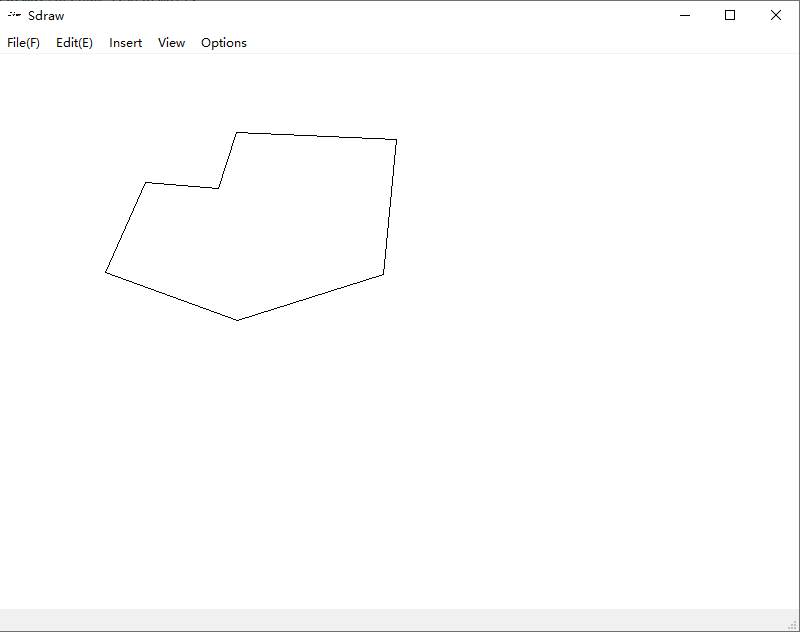
\includegraphics[width=6cm]{x7.png}   %以pic.jpg的0.5倍大小输出
	\end{minipage}
}
\subfigure[旋转90度后] %第二张子图
{
	\begin{minipage}[t]{0.35\linewidth}
	\centering      %子图居中
	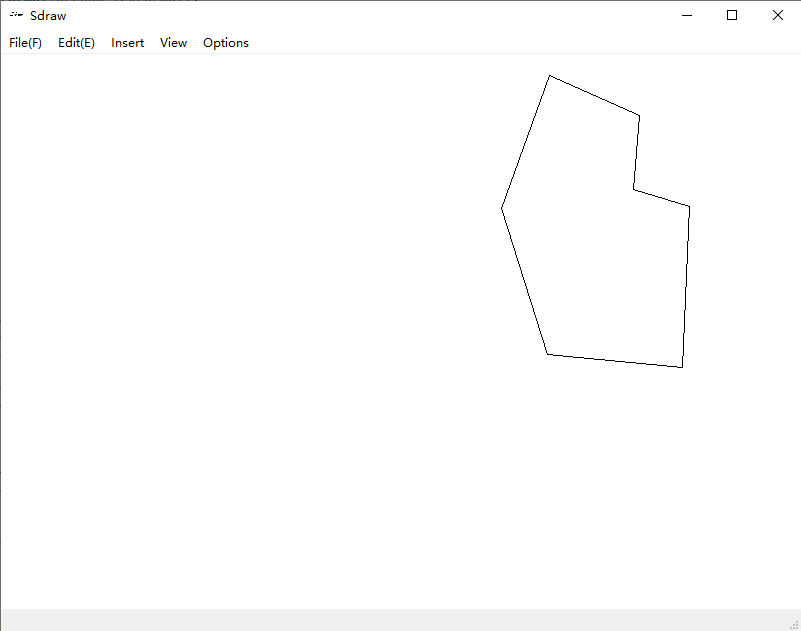
\includegraphics[width=6cm]{x8.png}   %以pic.jpg的0.5倍大小输出
	\end{minipage}
}
 
\caption{旋转算法 示意图} %  %大图名称
\label{x78}  %图片引用标记
\end{figure}

\subsection{缩放算法}
缩放算法类似于旋转算法,也是将点的坐标乘以矩阵,但是由于放大缩小点的数量不同,单纯的将图元中所有点乘矩阵会使得缩小时较小的面积上重复汇聚了较多的点,而放大时更大的空间上汇聚的点数依然与之前相同,导致图元上点过于稀疏,模糊不清,且多次放缩后会使得图元变形,所以我们采用类似旋转算法的方法,只对字典中图元的构造点集进行操作。公式如下:
\begin{equation}
\left\{
\begin{aligned}
x1=x*s_{x}+x_{f}*(1-s_{x})\\
y1=y*s_{x}+x_{f}*(1-s_{x})
\end{aligned}
\right.
\end{equation}
\begin{figure}[htbp]
\centering    %居中
 
\subfigure[原图] %第一张子图
{
	\begin{minipage}[t]{0.35\linewidth}
	\centering          %子图居中
	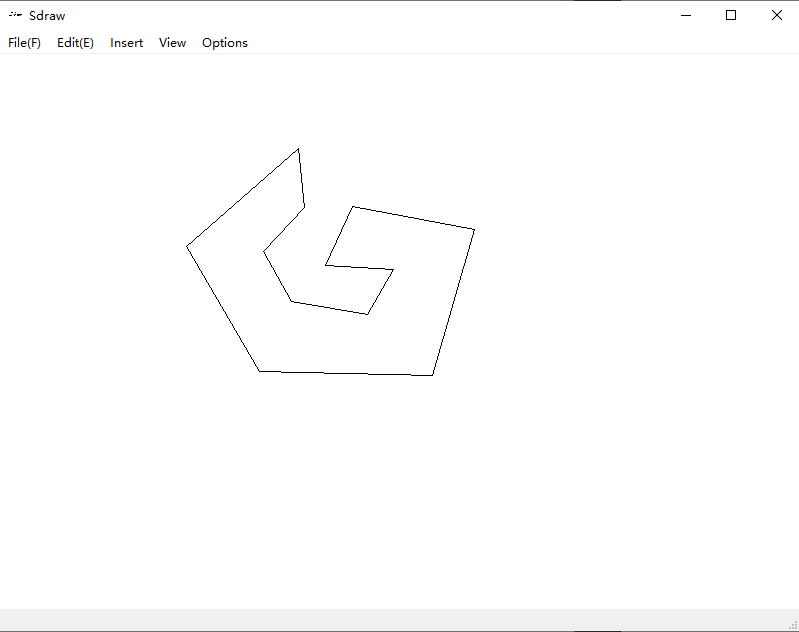
\includegraphics[width=6cm]{x9.png}   %以pic.jpg的0.5倍大小输出
	\end{minipage}
}
\subfigure[缩放0.5后] %第二张子图
{
	\begin{minipage}[t]{0.35\linewidth}
	\centering      %子图居中
	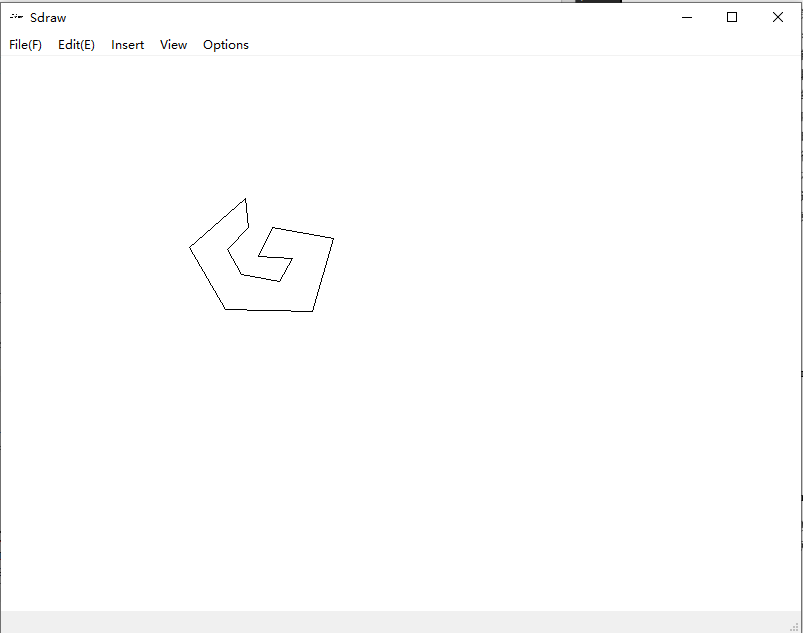
\includegraphics[width=6cm]{x10.png}   %以pic.jpg的0.5倍大小输出
	\end{minipage}
}
 
\caption{缩放算法 示意图} %  %大图名称
\label{x910}  %图片引用标记
\end{figure}

\section{系统介绍}
\subsection{系统架构}
系统基于Qt gui设计完成了软件。主要分为两个模块,一个是主窗口模块,一个是图形库模块。
\par 主窗口模块主要完成了gui的交互功能,图形库则主要完成了图元的绘制,包含了软件的各种操作。
\par 主要思想是利用QOpenGLWidget自带的三个函数,paintGL,initializeGL,resizeGL, 来完成图元的显示,图元在机器上存储在一个QVector中,Vector采用的模板是自定义的Point类型,类型中有choosen作为flag来标识是否被选中,pid表示所在图元的编号,size表示画这一点时其大小,mode表示其是在什么图元绘制模式下被绘制的。color数组表示了其颜色的RGB。x,y表示了其所在位置。
\par paintGL在软件中负责将Vector中存储的数据画出。
\par 图元绘制的基本函数则是点的绘制,注意在这里绘制指的是将Point对象存储到QVector中。基于点绘制的高级图元绘制则在之前的算法中已经涉及。
\par 之后还涉及一些简单的系统功能的实现,如选中,我设计了当按下中键时取消所在绘制状态改为选择状态,此时当鼠标的位置在一个图元的像素附件,则求出此像素所归属图元并求出图元pid,再搜索所有pid与此pid相等的点,将choosen即flag一一标志为真。当用户点到无像素地区,则在一般软件中,将取消选中,所以我们也采用了此类逻辑。被选中的图元在显示时颜色变灰,并可以进行编辑一栏中的操作,如删除(可以按快捷键)。
\par 于此同时还实现了文档读取软件开始绘制已实现功能,保存画布等功能。具体操作等详见使用手册。

\end{document}